\chapterimage{slike/Laguerre.jpg} % Chapter heading image

\chapter{Koherentni snopi svetlobe}
V tem poglavju bomo zapisali obosni približek valovne enačbe in spoznali 
njeno osnovno rešitev: Gaussov snop. Obravnavali bomo snope osnovnega in višjega reda ter
se naučili računati prehode Gaussovih snopov prek optičnih elementov. 

\section{Omejen snop svetlobe}
Pri obravnavi elektromagnetnega valovanja pogosto uporabljamo
približek ravnih valov\index{Ravni val}. Ti so v smeri pravokotno na smer širjenja
neomejeni in so zato lahko le idealizacija. Čim raven val usmerimo skozi odprtino
v zaslonu, dobimo omejen snop svetlobe\index{Omejen snop}. V snopu svetlobe valovna čela niso
ravna in meje snopa niso vzporedne, ampak se snop zaradi uklona širi (slika \ref{fig:Uklon-na-rezi}).
\begin{figure}[h]
\centering
\def\svgwidth{120truemm} 
\input{slike/03_uklon_na_rezi.pdf_tex}
\caption{Omejen snop dobimo ob prehodu ravnega vala skozi končno odprtino.}
\label{fig:Uklon-na-rezi}
\end{figure}

V veliki oddaljenosti od zaslona lahko za izračun polja uporabimo
\index{Fraunhoferjev uklon}Fraunhoferjevo uklonsko teorijo (glej poglavje~\ref{FFuklon}). 
Vendar za oceno kota širjenja podrobnega računa niti ne potrebujemo. Velja približno 
\begin{equation}
\vartheta\sim\frac{\lambda}{a},
\label{eq:kot_ocena}
\end{equation}
kjer je $a$ polmer odprtine v zaslonu.
Opis polja v bližini zaslona je zahtevnejši, saj je treba uporabiti 
Fresnelov približek\index{Fresnelov uklon}. S slike (\ref{fig:Uklon-na-rezi})
ocenimo, da seže območje bližnjega polja do razdalje 
\begin{equation}
b\sim\frac{a}{\vartheta}=\frac{a^{2}}{\lambda}.
\label{eq:z_ocena}
\end{equation}

Včasih taki približni oceni zadoščata. Bolj kvantitativen opis omejenih
snopov bi lahko dobili s Fraunhoferjevo in Fresnelovo uklonsko teorijo,
kar pa ni najudobnejša pot. Lotimo se naloge raje preko približka
obosne valovne enačbe.

\begin{definition}
Pokaži, da je Fraunhoferjeva uklonska slika reže, katere prepustnost se v radialni smeri
spreminja kot Gaussova funkcija $T(\xi, \eta)=e^{-(\xi^2+\eta^2)/w_0^2}$, podana z Gaussovo funkcijo
oblike $E(x,y,z) \propto e^{-(x^2+y^2)/w^2(z)}$ in dolo\v ci odvisnost $w(z)$. Izračunaj še 
uklonsko sliko v bližnjem polju po Fresnelovi uklonski teoriji.
\end{definition}

\section{Obosna valovna enačba}
Pričnimo s časovno neodvisno valovno enačbo za monokromatsko valovanje
s frekvenco $\omega$, to je \index{Helmholtzeva enačba}Helmholtzevo enačbo (enačba~\ref{eq:Helmholtz})
\begin{equation}
\nabla^{2}E+k^{2}E=0,
\label{eq:valovna-enacba-hh}
\end{equation}
kjer je $k=n\omega/c_{0}$ valovno število in $n$ lomni količnik
sredstva, po katerem se valovanje širi. Zaradi enostavnosti obravnavajmo
le eno polarizacijo, tako da $E$ pišemo kot skalar. Iščemo rešitev za
omejen snop, ki se širi približno vzdolž osi $z$. Zapišimo jo v obliki
\begin{equation}
E=E_{0}\psi(\mathbf{r},z)e^{ikz},
\label{eq:ravni-val-nastavek}
\end{equation}
kjer je $\mathbf{r}$ krajevni vektor v ravnini $xy$. Glavni del odvisnosti
od koordinate $z$ smo zapisali v faktorju $e^{ikz}$, tako da lahko
privzamemo, da se $\psi$ v smeri $z$ le počasi spreminja. Vstavimo
gornji nastavek v Helmholtzevo enačbo (\ref{eq:valovna-enacba-hh})
in pri tem zanemarimo druge odvode po $z$, saj je zaradi počasnega spreminjanja
$\partial^{2}\psi/\partial z^{2}$ majhen v primerjavi s $k\partial\psi/\partial z$ in $k^{2}\psi$.
Zaenkrat obravnavajmo le radialno simetrične rešitve. Dobimo obosno
ali paraksialno valovno enačbo\index{Obosna valovna enačba}
\boxeq{eq:obosna-valovna-enacba}{
\nabla_{\perp}^{2}\psi=-2ik{\frac{{\partial\psi}}{{\partial z}}}.
}
Opazimo, da je obosna valovna enačba enaka Schr\"{o}dingerjevi enačbi
za prost delec v dveh dimenzijah, v kateri ima koordinata $z$ vlogo
časa. Omejenemu snopu v kvantni mehaniki ustreza lokaliziran delec
-- valovni paket. Ta se s časom širi, kar v optiki ustreza pojavu uklona.

Ena družina rešitev, ki v kvantni mehaniki predstavlja lastne funkcije
energije in gibalne količine, so ravni valovi\index{Ravni val}
\begin{equation}
\psi=e^{ik_{1}x+ik_{2}y}\, e^{-i\beta z}.
\label{eq:ravni-val-nastavek-obosni}
\end{equation}
Pri tem $\beta$ ustreza energiji v kvantni mehaniki, $k_{1}$ in
$k_{2}$ pa komponentama gibalne količine. Da bo gornji nastavek rešitev
obosne valovne enačbe~(\ref{eq:obosna-valovna-enacba}), mora veljati 
\begin{equation}
\beta=\frac{k_{1}^{2}+k_{2}^{2}}{2k}.
\end{equation}
Ko vstavimo nastavek za $\psi$ v izraz za celotno polje $E$ 
(enačba~\ref{eq:ravni-val-nastavek}), dobimo ravni val\index{Ravni val}, za katerega velja 
\begin{equation}
k_{3}=k-\beta=k-\frac{k_{1}^{2}+k_{2}^{2}}{2k},\label{eq:k3-razvoj}
\end{equation}
 pri čemer je $k_{3}$ vzdolžna komponenta valovnega vektorja, $k_{1}$ in
$k_{2}$ prečni komponenti, $k$ pa valovno število. 

Za ravni val, ki je rešitev prvotne točne valovne enačbe (\ref{eq:valovna-enacba-hh})
in ne samo obosnega približka, velja 
\begin{equation}
k_{3}=\sqrt{k^{2}-(k_{1}^{2}+k_{2}^{2})}.\label{eq:k3-tocno}
\end{equation}
Očitno dobimo enačbo~(\ref{eq:k3-razvoj}) iz enačbe~(\ref{eq:k3-tocno})
z razvojem korena za majhne vrednosti prečnih komponent valovnega
vektorja, kar seveda ni nič nepričakovanega. Ta ugotovitev nam tudi
pove, da je približek obosne enačbe dober, kadar je razmerje prečne
in vzdolžne komponente valovnega vektorja majhno. Takrat je majhen
tudi kot širjenja snopa in v razvoju lahko zanemarimo člene, višje
od kvadratnih. To pa je tudi območje veljavnosti Fresnelove uklonske
teorije, zato rešitve obosne valovne enačbe dajo enako dober približek.

\begin{remark}{{\bf Fouriereva optika}}\\ \\
Časovno odvisnost poljubnega začetnega
stanja v kvantni mehaniki navadno izračunamo tako, da v nekem začetnem
trenutku paket razvijemo po lastnih stanjih energije -- ravnih valovih.
Rešitev v poljubnem kasnejšem trenutku je potem dana v obliki Fourierevega
integrala. Ta pot je zelo uporabna tudi v optiki in je osnova sklopa
računskih metod, znanih pod imenom Fouriereva optika. V našem primeru
z njo brez težav pridemo nazaj do Fresnelove uklonske formule.
\end{remark}

\section{Osnovni Gaussov snop}
Naša naloga je poiskati rešitve obosne enačbe, ki popišejo omejene
snope. Iz kvantne mehanike vemo, da je najbolj lokaliziran in se najpočasneje
širi valovni paket Gaussove oblike. Zato poskusimo najti rešitev obosne
enačbe (\ref{eq:obosna-valovna-enacba}) v obliki 
\begin{equation}
\psi(r,z)=e^{i\frac{kr^{2}}{2q(z)}}\, e^{-i\phi(z)},\label{eq:gaussov-snop-nastavek}
\end{equation}
kjer funkcija $q(z)$ opisuje širjenje snopa v prečni smeri,
$\phi(z)$ pa opisuje počasno spreminjanje faze snopa vzdolž osi $z$.
Vstavimo nastavek (enačba~\ref{eq:gaussov-snop-nastavek}) v enačbo~(\ref{eq:obosna-valovna-enacba}).
Zaradi simetričnosti računamo v cilindričnih koordinatah in zapišemo
\begin{equation}
\nabla_{\perp}^{2}\psi=\frac{1}{r}\frac{\partial}{\partial r}\, r\,\frac{\partial\psi}{\partial r}=
\left( \frac{2ik}{q}-\frac{k^2r^2}{q^2}\right)\psi
\end{equation}
 in 
\begin{equation}
\frac{\partial\psi}{\partial z}=\left(-\frac{ikr^{2}}{2q^2}q(z)^{\prime}-i\phi^{\prime}\right)\psi.
\end{equation}
Tako iz obosne enačbe (\ref{eq:obosna-valovna-enacba}) dobimo
\begin{equation}
\frac{2ik}{q}-\frac{k^2r^2}{q^2}=ik\left(\frac{ikr^{2}}{q^2}q(z)^{\prime}+2i\phi^{\prime}\right).
\end{equation}
Gornji izraz mora veljati pri vsakem $r$, zato morajo biti koeficienti
pri $r^{2}$ in pri drugih členih posebej enaki 0. Dobimo
\begin{equation}
q(z)^{\prime}=1\mbox{\hskip1cm in \hskip1cm}\phi^{\prime}=-\frac{i}{q}.
\end{equation}
 Z integracijo dobimo najprej 
\begin{equation}
q=z-iz_{0},
\label{eq:alpha}
\end{equation}
kjer smo z $i z_{0}$ označili integracijsko konstanto. 
Integriramo še enačbo za fazo 
\begin{equation}
\phi=\int_{0}^{z}\,-\frac{i dz}{z-iz_{0}}=-i\ln(1+i\frac{z}{z_{0}}).
\end{equation}
Tako imamo 
\begin{eqnarray}
\psi & = & \exp\left[i\frac{kr^{2}}{2(z-iz_0)}\right]\,\exp\left[-\ln(1+i\frac{z}{z_{0}})\right]=
\nonumber \\
 & = & \frac{1}{1+i\frac{z}{z_{0}}}\,\exp\left[-\frac{kr^{2}z_{0}}{2(z_{0}^{2}+z^{2})}+
 \frac{ikr^{2}z}{2(z_{0}^{2}+z^{2})}\right].
 \label{eq:gaussov-snop-vmesni}
\end{eqnarray}
Realni del eksponenta opisuje širjenje snopa. Vpeljimo polmer snopa\index{Gaussov snop!polmer}
$w$: 
\begin{equation}
w^{2}=\frac{2z_{0}}{k}\left[1+\left(\frac{z}{z_{0}}\right)^{2}\right].
\end{equation}
V izhodišču pri $z=0$ je snop najožji in pravimo, da je tam grlo snopa\index{Gaussov snop!grlo}. 
Vpeljimo še polmer snopa v grlu $w_0$ in zapišimo hiperbolično odvisnost $w$ od $z$:
\boxeq{eq:w}{
w^2 = w_{0}^{2}\left[1+\left(\frac{z}{z_{0}}\right)^{2}\right].
}
Med $w_{0}$ in $z_{0}$ velja zveza 
\boxeq{eq:z0}{
z_{0}=\frac{\pi w_{0}^{2}}{\lambda}.
}
Dolžina $z_{0}$ je ravno razdalja, pri kateri preide snop v asimptotično enakomerno širjenje.
Pri $z_{0}$ tudi preidemo v območje veljavnosti Fraunhoferjevega uklonskega približka. 
Celotna dolžina grla je $2z_0$, območju grla pa pravimo tudi območje bližnjega polja ali 
Rayleighovo območje in dolžini $z_0$ \index{Rayleighova dolžina}Rayleighova 
dolžina\footnote{Angleški fizik in nobelovec John William Strutt, 3. baron Rayleighški, 1842--1919.}.

\begin{figure}[h]
\centering
\def\svgwidth{100truemm} 
\input{slike/03_Gauss.pdf_tex}
\caption{Gaussov snop s karakterističnimi parametri}
\label{fig:Gauss}
\end{figure}

Iz izraza (\ref{eq:w}) za polmer snopa $w(z)$ razberemo še kot divergence snopa v
asimptotičnem območju. Najprej izračunajmo le polovični kot širjenja:
\begin{equation}
\vartheta=\lim_{z \to \infty} \frac{dw}{dz} = \frac{w_{0}}{z_{0}}=\frac{\lambda}{\pi w_{0}}.\label{eq:divergenca-snopa}
\end{equation}
Nato pa zapišimo celotno divergenco snopa\index{Divergenca snopa}
\boxeq{eq:divergenca-snopa2}{
\theta=2 \frac{w_{0}}{z_{0}}=\frac{2\lambda}{\pi w_{0}}.
}

Dobljena izraza za območje bližnjega polja (enačba~\ref{eq:z0}) in divergenco 
(enačba~\ref{eq:divergenca-snopa}) sta v skladu z grobimi ocenami, ki smo jih 
napravili v začetku poglavja (enačbi~\ref{eq:kot_ocena} in \ref{eq:z_ocena}). Faktor 
$1/\pi$ je značilen za Gaussov snop, ki ima od vseh mogočih oblik 
najmanjšo divergenco.

Vrnimo se k imaginarnemu delu eksponenta v drugi enačbi~(\ref{eq:gaussov-snop-vmesni}).
Vpeljimo količino 
\boxeq{eq:R}{
R=z\left[1+\left(\frac{z_{0}}{z}\right)^{2}\right],
}
ki meri krivinski radij valovnih front snopa na razdalji $z$. To najlažje
uvidimo, če krogelni val razvijemo po majhnih odmikih $r$ od osi
$z$: 
\begin{equation}
\frac{1}{R}e^{ikR}=\frac{1}{R}e^{ik\sqrt{z^{2}+r^{2}}}\simeq\frac{1}{R}e^{ik(z+\frac{r^{2}}{2R})}.\label{eq:krogelni-val}
\end{equation}
 Upoštevali smo, da je na osi $z=R$.

\begin{definition}
\label{naloga-ukrivljenost-snopa}
Pokaži, da je največja ukrivljenost valovnih front snopa (najmanjši $R$) ravno pri $z=\pm z_{0}$.
Izračunaj še ukrivljenost front v grlu in v veliki oddaljenosti od grla.
\end{definition}
 
Ostane nam še faktor pred eksponentom v izrazu~(\ref{eq:gaussov-snop-vmesni}). Ta faktor meri
zmanjševanje amplitude snopa in s tem poskrbi za ohranitev energijskega
toka ob širjenju žarka, poleg tega pa da še dodatno spremembo faze. Zapišimo ga v obliki
\begin{equation}
\frac{1}{1+i\frac{z}{z_{0}}}=\frac{1}{\sqrt{1+(\frac{z}{z_0})^{2}}}e^{-i\eta(z)}=\frac{w_{0}}{w}e^{-i\eta(z)},
\end{equation}
 pri čemer je
\boxeq{eq:eta}{
\eta(z)=\arctan(\frac{z}{z_{0}}).
}
Dodatna faza $\eta$, imenujemo jo tudi \index{Gouyeva faza}Gouyeva 
faza\footnote{Francoski fizik Louis Georges Gouy, 1854--1926.}
je posledica povečane fazne hitrosti valovanja,
kadar je omejeno v prečni smeri. Pojav je najizrazitejši v bližini
grla snopa. Srečamo ga tudi pri valovanju v valovodih.

S tem lahko končno zapišemo izraz za električno poljsko jakost osnovnega Gaussovega snopa\index{Gaussov snop}
\boxeq{eq:gaussov-snop}{
E=E_{0}\,\frac{w_{0}}{w(z)}\,e^{ikz-i\omega t}\,e^{-r^{2}/w^{2}(z)}\,e^{ikr^{2}/2R(z)}
e^{-i\eta(z)}.
}
Intenziteta svetlobe je sorazmerna z $E(r,z)E^*(r,z)$ in zanjo velja
\boxeq{eq:gaussov-snop-intenziteta}{
I(r,z)= I_{0}\,\frac{w_0^2}{w(z)^2}\,e^{-2r^{2}/w^{2}(z)}.
}

\begin{figure}[h]
\centering
\def\svgwidth{110truemm} 
\input{slike/03_Gauss_3D.pdf_tex}
\caption{Upodobitev gostota svetlobnega toka v Gaussovem snopu za $z>0$. }
\label{fig:Gauss_3D}
\end{figure}

\begin{definition}
\label{naloga-širina-snopa}
Pokaži, da je znotraj širine snopa $w$ približno $87~\%$ celotnega svetlobnega toka.
\end{definition}

Povejmo še nekaj o parametru $q(z)$, ki smo ga uporabili pri izračunu Gaussovega snopa. Spom\-nimo 
se, da parameter $q$ narašča linearno z oddaljenostjo od grla:
\boxeq{eq:q}{
q(z) = z -iz_0.
}
Parameter $q$ imenujemo kompleksni krivinski radij\index{Kompleksni krivinski radij}, 
njegov inverz pa kompleksna ukrivljenost\index{Kompleksna ukrivljenost}: 
\boxeq{eq:q-inv}{
\frac{1}{q(z)}=\frac{1}{R}+i\frac{2}{kw^{2}}.
}

Primerjajmo še Gaussov snop z drugimi valovanji. Na sliki (\ref{fig:ravni-Gaussov-krogelni-val}) 
so shematsko prikazane valovne fronte ravnega vala, Gaussovega snopa (\ref{eq:gaussov-snop}) in krogelnega
vala (\ref{eq:krogelni-val}). Vidimo, da je za majhne oddaljenosti od grla $z$ Gaussov
snop podoben ravnemu valu (ukrivljenost front je zelo majhna in $R \to \infty$), 
medtem ko je za velike $z$ podoben krogelnemu valu (krivinski radij $R$ narašča sorazmerno z oddaljenostjo $z$). 
Faza Gaussovega snopa je pri pri $z\gg z_{0}$ zamaknjena za $\pi/2$ glede na ravni in 
krogelni val. 

\begin{figure}[h]
\centering
\def\svgwidth{100truemm} 
\input{slike/03_fronte.pdf_tex}
\caption{Ravni val, Gaussov snop ter
krogelni val. Pri majhnih razdaljah od grla je Gaussov snop podoben
ravnemu valu, pri velikih razdaljah pa krogelnemu valu. Faza Gaussovega snopa
se razlikuje od faze ravnega in krogelnega vala.}
\label{fig:ravni-Gaussov-krogelni-val}
\end{figure}

\section{Snopi višjega reda}

Osnovna rešitev obosne valovne enačbe je Gaussov snop. Poleg te rešitve pa obstoja še veliko 
drugih rešitev, ki so tudi omejene v prečni smeri. V kartezičnih koordinatah tako rešijo obosno valovno enačbo
tudi Hermite-Gaussovi snopi\index{Hermite-Gaussovi snopi}
\begin{equation}
\psi_{n,m}(x,y)=\frac{w_{0}}{w}H_{n}\left(\frac{\sqrt{2}x}{w}\right)H_{m}\left(\frac{\sqrt{2}y}{w}\right)
\exp\left[\frac{ik(x^{2}+y^{2})}{2q}-i\eta_{n,m}\right],
\label{eq:Gauss-Hermitevi}
\end{equation}
kjer so $H_{n}$ Hermitovi polinomi stopnje $n$. V to se lahko
prepričamo, če izraz vstavimo v obosno enačbo (\ref{eq:obosna-valovna-enacba}) in upoštevamo, 
da Hermitovi polinomi zadoščajo enačbi 
\begin{equation}
H_{n}^{\prime\prime}-2xH_{n}^{\prime}+2nH_{n}=0.
\end{equation}
Osnovni Gaussov snop je očitno poseben primer gornje rešitve za $m=n=0$.
Polmer snopa $w(z)$ in kompleksni krivinski radij $q(z)$ sta za
vse $m$ in $n$ enaka kot za osnovni snop in podana z enačbama (\ref{eq:w})
in (\ref{eq:q}). Razlika je v fazi, ki je odvisna tudi od $n$ in $m$: 
\begin{equation}
\eta_{n,m}\left(z\right)=(n+m+1)\arctan\left(\frac{z}{z_{0}}\right).
\end{equation}
To hitrejše spreminjanje faze v bližnjem polju snopov višjega reda
je analogno večji fazni hitrosti valov višjega reda v valovodih.

Nekaj višjih redov Hermite-Gaussovih snopov je na sliki (\ref{fig:Gauss-Hermitevi-snopi}),
kjer rišemo $|\Re\psi_{n,m}(x, y, 0)|$.
Vidimo, da indeksa $n$ in $m$ predstavljata število vozlov v prečni smeri,
pri danem $w$ pa polmer snopa narašča z $n$ in $m$. 

\begin{figure}[h]
\centering
\def\svgwidth{120truemm} 
\input{slike/03_Hermite_Gauss.pdf_tex}
\caption{Prečni profil Hermite-Gaussovih snopov za različne vrednosti $(n,m)$.}
\label{fig:Gauss-Hermitevi-snopi}
\end{figure}

\begin{definition}
\label{naloga:HG}
Pokaži, da za Hermite-Gaussove snope višjih redov efektivni polmer snopa 
narašča sorazmerno s korenom iz števila prečnih vozlov $ w_{eff}\propto w\sqrt{n+m}$.
Namig: pri zapisu prečne odvisnosti polja upoštevaj le vodilni člen
 Hermitovih polinomov ($\psi_{n,m}\propto x^{n}y^{m}\exp(-(x^{2}+y^{2})/w^{2})$)
 in določi, na kateri razdalji od središča snopa ima polje $\psi$
največjo amplitudo.
\end{definition}

Hermite-Gaussovi snopi (\ref{eq:Gauss-Hermitevi}) tvorijo popoln
ortogonalen sistem funkcij koordinat $x$ in $y$:
\begin{equation}
\int\psi_{n,m}^{*}(x,y)\psi_{n',m'}(x,y)\, dx dy=\pi w_{0}^{2}\; 
2^{n+m-1}n!\;m!\; \delta_{n,n'}\;\delta_{m,m'}
\end{equation}
Polje nekega valovanja, ki ga poznamo v ravnini $z=0$, lahko pri
poljubnem $z$ dobimo z razvojem po Hermite-Gaussovih snopih. Pri tem
je izbira premera grla $w_{0}$ poljubna, bo pa seveda vplivala na
hitrost konvergence razvoja. Na tak način lahko obravnavamo uklon
na odprtini, kjer je očitno smiselno vzeti $w_{0}$ približno enak
dimenziji odprtine. Dobljeni rezultat je enako natančen kot Fresnelov
uklonski integral.

Pri velikih $z$, kjer velja Fraunhoferjeva uklonska teorija, je
polje Fouriereva transformacija polja pri $z=0$. Hermite-Gaussovi
snopi ohranjajo prečno obliko, ki pa se z naraščajočim $z$ širi. 
Od tod vidimo, da je Fouriereva transformacija Hermite-Gaussove funkcije 
$H_{n}(x)e^{-x^{2}/2}$ zopet Hermite-Gaussova funkcija.

V cilindričnih koordinatah imajo snopi višjega reda obliko Laguerre-Gaussovih 
snopov\index{Laguerre-Gaussovi snopi}
\begin{equation}
\psi_{p,l}(r,\phi,z)=\frac{w_{0}}{w}\left(\frac{\sqrt{2}r}{w}\right)^{|l|}
L_{p}^{|l|}\left(\frac{2r^{2}}{w^{2}}\right)e^{\pm il\phi}\exp\left[\frac{ikr^{2}}{2q}-i\eta_{p,l}\right],
\label{eq:Gauss-Laguerrevi}
\end{equation}
kjer je $L_{p}^{l}$ pridruženi Laguerrov polinom in 
\beq
\eta_{p,l}\left(z\right)=(2p+l+1)\arctan\left(\frac{z}{z_{0}}\right).
\label{eq:etaGL}
\eeq

Podobno kot je v kartezičnem primeru red polinoma določal število prečnih ničel,
določata $p$ in $l$ v cilindričnem primeru število vozelnih črt, kjer je gostota 
svetlobnega toka nič. Na sliki~(\ref{fig:Laguerrovi_presek})
je prikazanih nekaj oblik amplitud $|\Re\psi_{p,l}(r,\phi,0)|$.

\begin{figure}[h]
\centering
\def\svgwidth{120truemm} 
\input{slike/03_Laguerre_Gauss.pdf_tex}
\caption{Prečni profil Laguerre-Gaussovih snopov za različne vrednosti $(p,l)$.}
\label{fig:Laguerrovi_presek}
\end{figure}

Iz laserjev navadno želimo dobiti čim čistejši osnovni snop, vendar
lahko pogosto opazimo tudi snope višjega reda. Da dobimo le osnovni
snop, je treba posebej paziti pri konstrukciji laserja.

\begin{remark}{{\bf Tirna vrtilna količina in spin}}\\ \\
Valovne fronte Laguerre-Gaussovih snopov pri $l\ne0$ imajo obliko vijačnic. Poyntingov 
vektor pri njih ni vzporeden z osjo žarka, ampak ima komponento tudi v prečni smeri. Ta spreminja smer, 
zato pride do pojava vrtilne količine v smeri osi snopa in snop na snov deluje z navorom. 
Pravimo, da Laguerre-Gaussovi snopi nosijo t.i. tirno vrtilno količino\index{Tirna vrtilna količina}. 
V kvantni mehaniki funkcija $\psi_{p,l}$ predstavlja foton s tirno vrtilno količino $L = \hbar l$, 
medtem ko leva in desna cirkularna polarizacija predstavljata spin fotona. 
\begin{figure}[h]
\centering
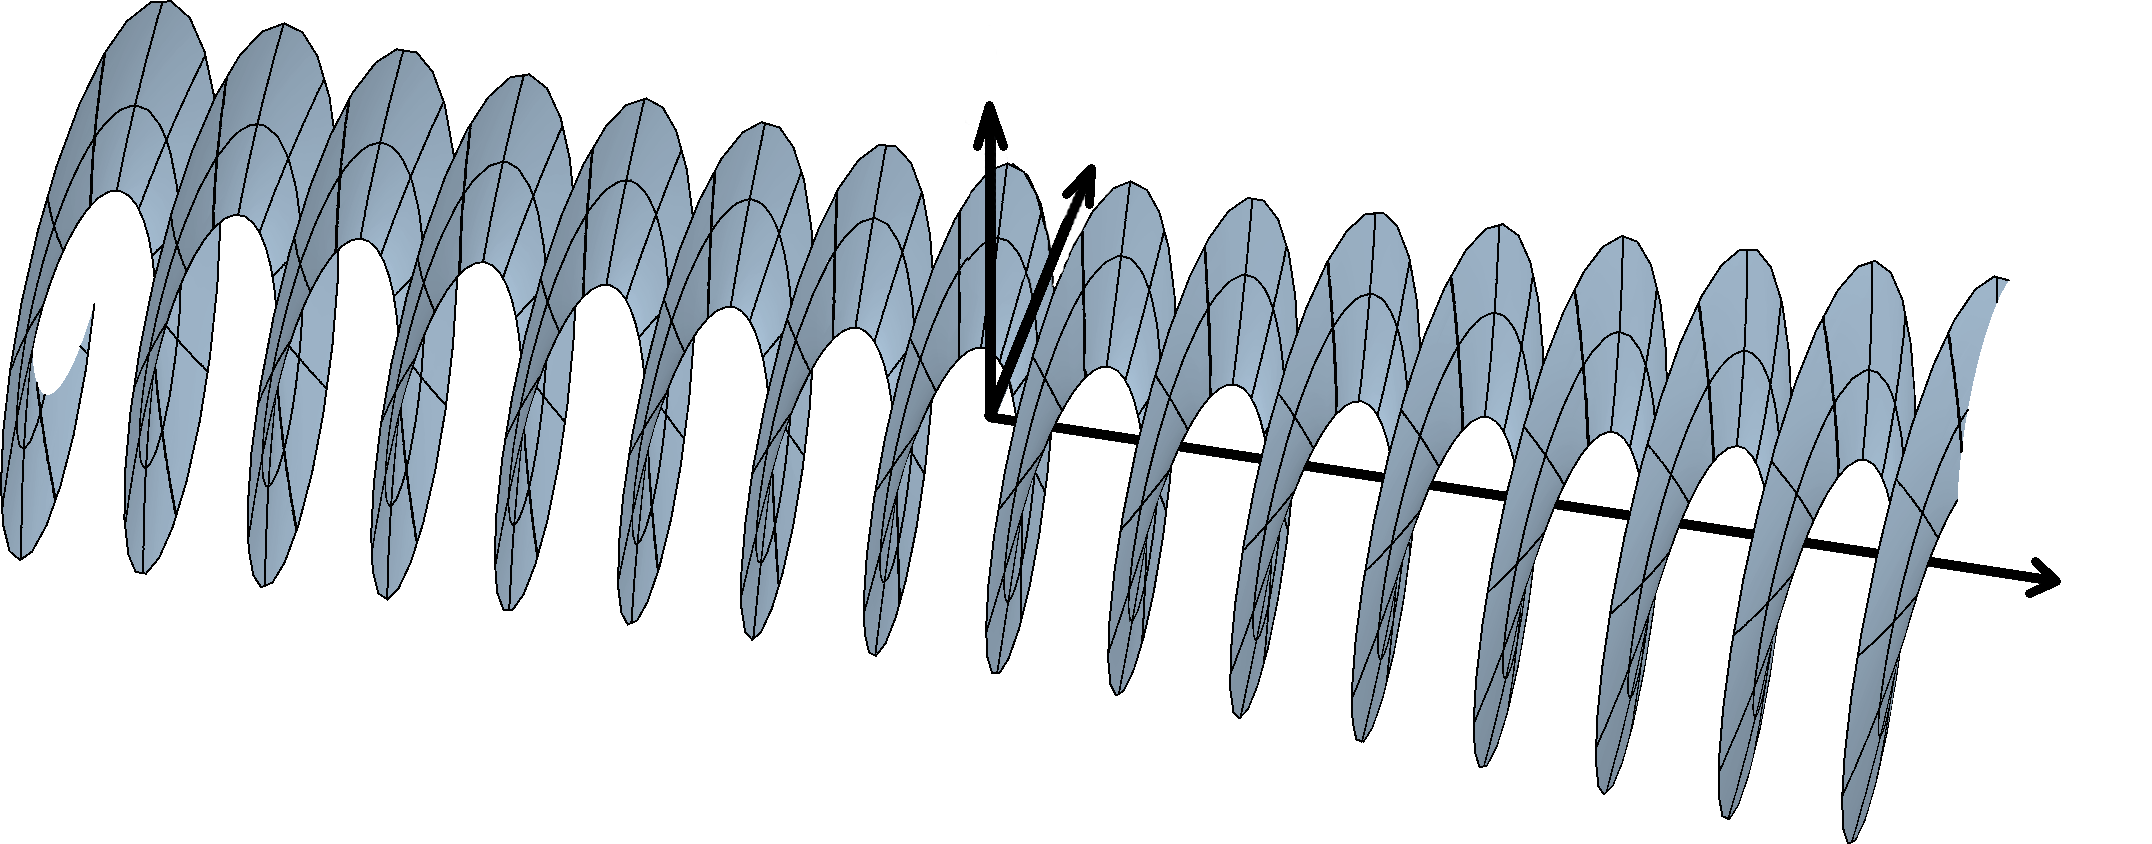
\includegraphics[width=10truecm]{slike/03_Laguerre_faza.png}
\caption{Valovna fronta Laguerre-Gaussovega snopa}
\label{fig:Laguerrova_fronta}
\end{figure}
\end{remark}

\section{Besselov snop}

Poglejmo si še poseben primer omejenega snopa, to je \index{Besselov snop}Besselov
snop\footnote{Nemški astronom, matematik in fizik Friedrich Wilhelm Bessel,1784--1846.}. 
Kot nastavek za rešitev valovne enačbe (\ref{eq:valovna-enacba-hh})
izberemo
\begin{equation}
E=E_{0}\psi(x,y)e^{i\beta z-i\omega t},
\end{equation}
kjer mora nastavek $\psi$ zadostovati Helmholtzovi enačbi
\begin{equation}
\nabla_{\perp}^{2}\psi+k_{\perp}^{2}\psi=0,
\end{equation}
pri $k_{\perp}^{2}=k^{2}-\beta^{2}$. V cilindričnih
koordinatah ($x=r\cos\phi$, $y=r\sin\phi$) se enačba prepiše v 
\beq
\frac{\partial^2 \psi}{\partial r^2}+ \frac{1}{r}\frac{\partial \psi}{\partial r}
+ \frac{1}{r^2}\frac{\partial^2 \psi}{\partial \phi^2}+k_{\perp}^{2}\psi=0.
\eeq
Rešitve gornje enačbe so s faznim faktorjem pomnožene Besselove funkcije:
\begin{equation}
\psi_m(x,y)=A_{m}J_{m}(k_{\perp}r)e^{im\phi},
\end{equation}
kjer je $J_{m}$ Besselova funkcija in $m=0,\pm1,\pm2 \ldots$ Za
$m=0$ ima val obliko
\begin{equation}
E(r,\phi,z,t)=A_{0}J_{0}(k_{\perp}r)e^{i\beta z-i \omega t},
\label{eq:Besselov-snop}
\end{equation}
ki ga imenujemo Besselov snop. Valovne fronte takega snopa so ravne 
in snop nima divergence. Vendar pa Besselov snop ni omejen v pravem smislu. Za 
velike oddaljenosti od središča snopa $r$ intenzitetni profil namreč pojema kot 
$I \propto J_{0}^{2}(k_{\perp}r)\approx(2/\pi k_{\perp}r)\cos^{2}(k_{\perp}r-\pi/4)$.
Energija takega snopa ni omejena znotraj efektivnega radija,
kot je to pri Gaussovih snopih. Za konstrukcijo Besselovih snopov
bi (tako kot za konstrukcijo ravnega vala) potrebovali neskončno energije,
kar je seveda nemogoče. Kljub temu pa lahko ustvarimo približke Besselovih 
snopov, ki imajo pomembne in uporabne lastnosti. 

\begin{figure}[h]
\centering
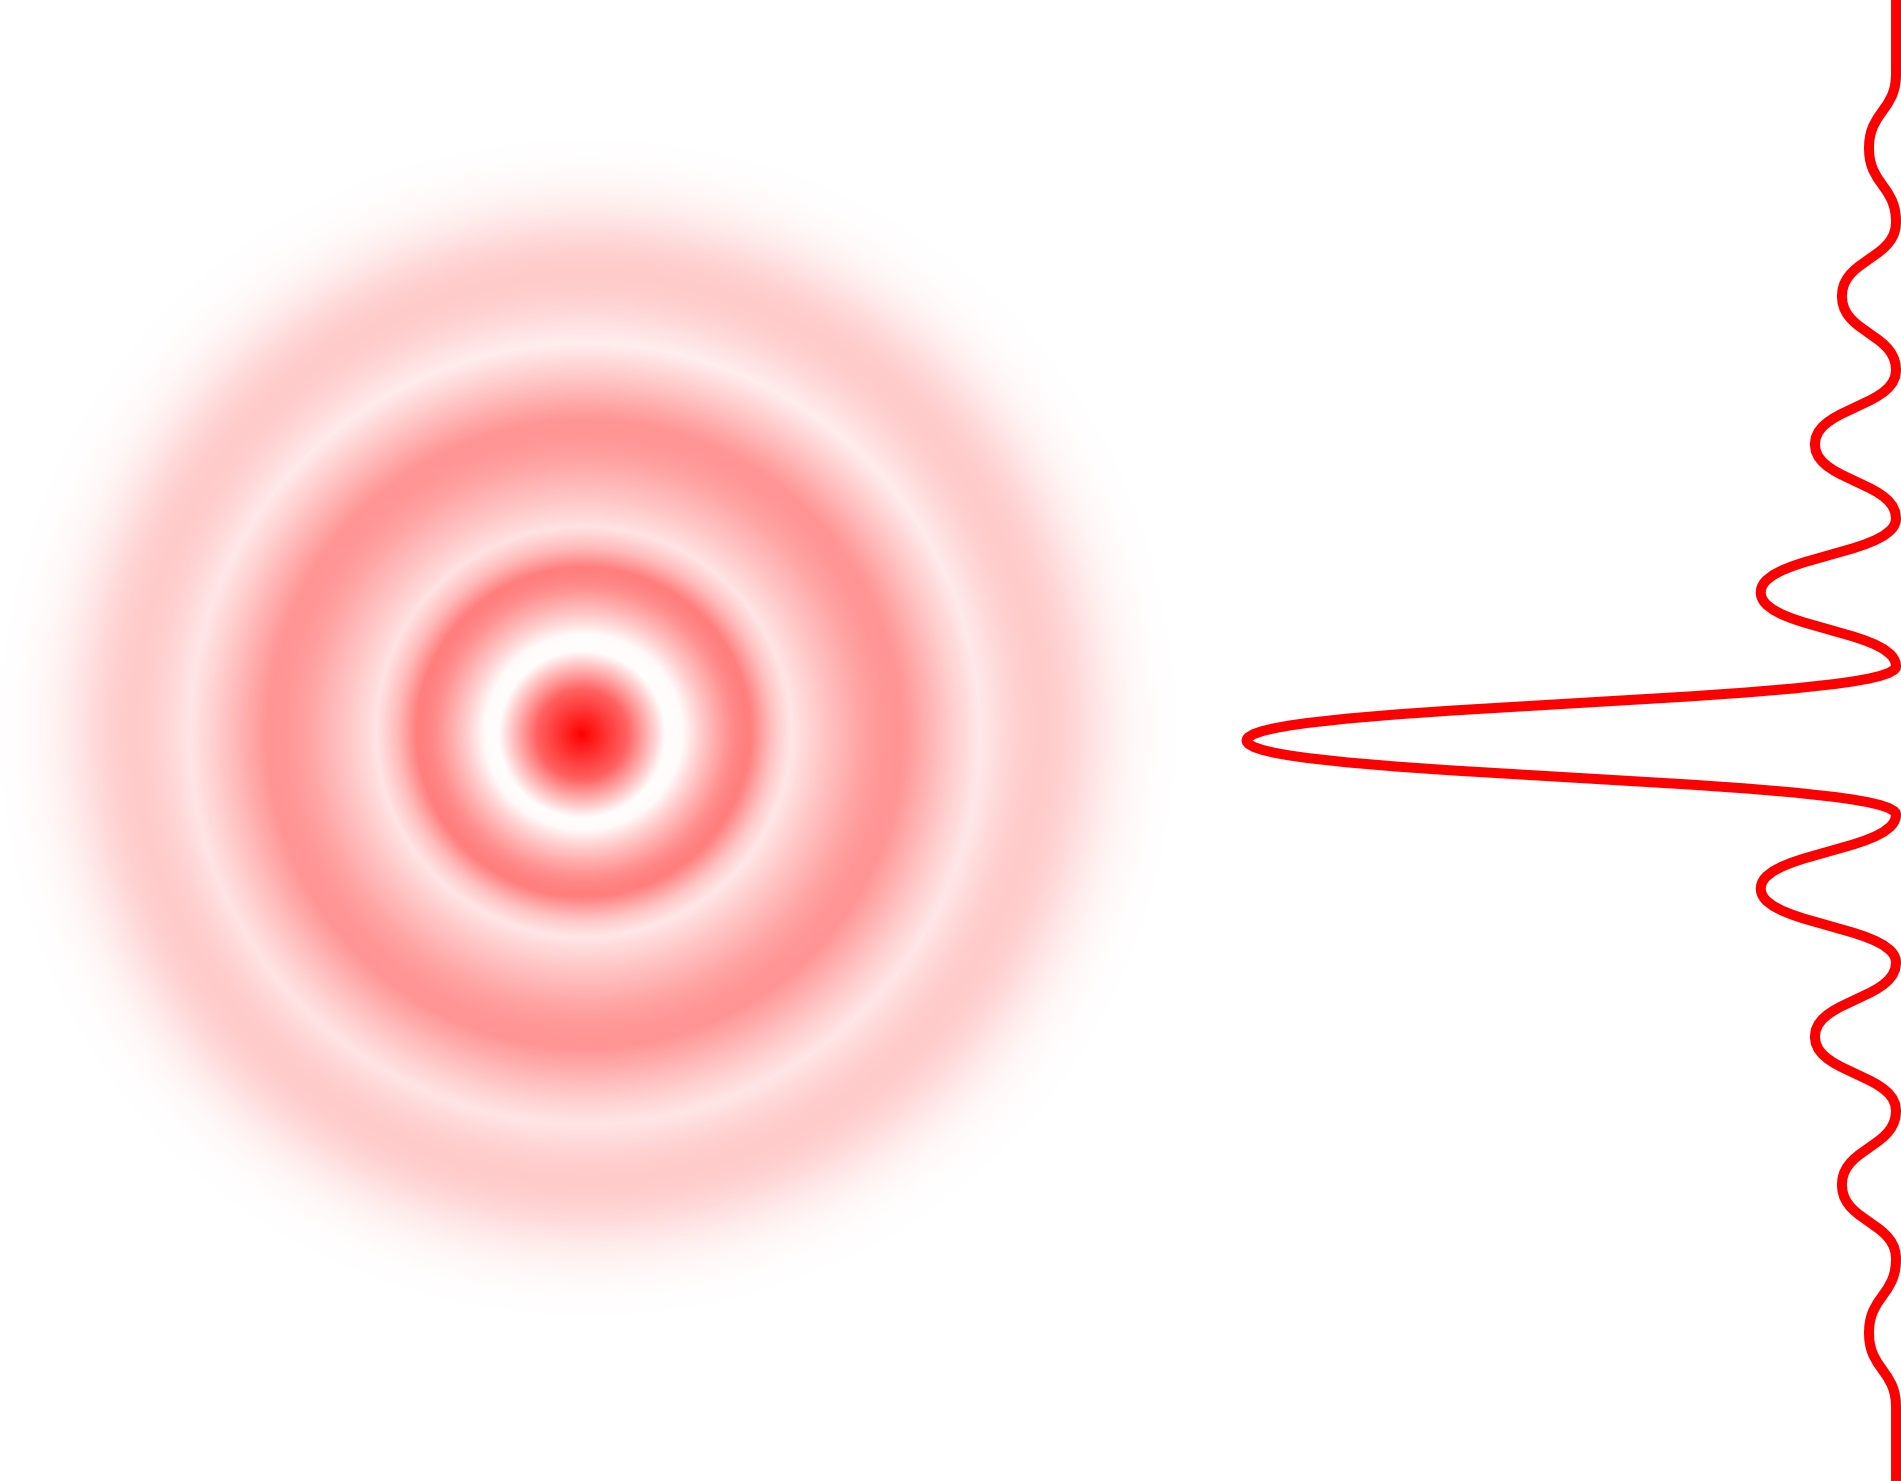
\includegraphics[width=7truecm]{slike/03_Bessel_profil.png}
\caption{Prečni presek in profil intenziteta Besselovega snopa}
\label{fig:Besselov_presek}
\end{figure}

\begin{remark}
Z uporabo stožčaste leče lahko Gaussov snop
preoblikujemo v približek Besselovega snopa (slika~\ref{fig:Bessel_leca}). 
Na plašču stožčaste leče se namreč Gaussov snop zlomi in valovni vektorji 
nastalega žarka opisujejo stožec, kar je sicer lastnost Besselovih žarkov.
Dobljeni žarek je približek Besselovega snopa, vendar le na določenem območju, dolgem $z_{max}$.
Znotraj tega območja je divergenca snopa praktično enaka nič. Poleg manjše divergence
imajo ti snopi še lastnost regeneracije. To pomeni, da se snop v senčni strani
za objektom, ki ga osvetljuje (na primer v optični pinceti), regenerira. 
Profil snopa v senčni strani (daleč stran od objekta) je tako enak profilu 
snopa pred objektom. 
\begin{figure}[h]
\centering
\def\svgwidth{100truemm} 
\input{slike/03_Bessel_nastanek.pdf_tex}
\caption{Nastanek Besselovega snopa na stožčasti leči.}
\label{fig:Bessel_leca}
\end{figure}
\end{remark}

\section{Transformacije snopov z lečami}

Vrnimo se h Gaussovim snopom in poglejmo, kaj se zgodi z njimi pri prehodu
skozi optične naprave\index{Preslikava čez lečo}. Začnimo
z enostavno tanko lečo z goriščno razdaljo $f$. V geometrijski optiki
je krivinski radij krogelnega vala, ki izhaja iz točke na osi, kar
enak razdalji do točke. Leča preslika točko na osi v točko na osi,
od tod pa sledi, da se sferični val s krivinskim radijem $R_{1}$
po prehodu skozi lečo spremeni v val s krivinskim radijem $R_{2}$.
Pri tem velja zveza 
\begin{equation}
\frac{1}{R_{1}}-\frac{1}{R_{2}}=\frac{1}{f}.
\end{equation}
Krivinski radij v točki $z$ je pozitiven, če je središče krožnice pri $z^{\prime}\le z$.

Kako pa je z Gaussovim snopom? Polmer snopa $w$ se pri prehodu 
skozi tanko lečo ne spremeni, zato velja po enačbi (\ref{eq:q-inv}) za
kompleksni krivinski radij tik pred lečo in tik za njo
\begin{equation}
\frac{1}{q_{1}}-\frac{1}{q_{2}}=\frac{1}{f}.
\label{eq:preslikava-zveza-leca}
\end{equation}
Kompleksni krivinski radij $q$ je po enačbi~(\ref{eq:q}) linearna funkcija koordinate $z$.
To nam skupaj z enačbo~(\ref{eq:preslikava-zveza-leca})
omogoča račun prehoda snopa skozi poljuben sistem leč brez aberacij.
Kot primer poglejmo, kako z zbiralno lečo zberemo snop.

Vpadni snop naj ima grlo s polmerom $w_{01}$ in parametrom $z_{01}$. Lega grla je 
v točki, ki je za $x_{1}$ oddaljena od levega gorišča leče (slika
\ref{fig:Prehod-Gaussovega-snopa}). Izračunati želimo položaj in
polmer grla na desni strani leče. Naj bosta 
\begin{equation}
q_{1}^{F}=x_{1}-iz_{01}\mbox{\hskip1cm in \hskip1cm}q_{2}^{F}=-x_{2}-iz_{02}
\end{equation}
 kompleksna krivinska radija v levem in desnem gorišču, pri čemer je koordinatna os $z$ 
 usmerjena v desno, gledamo pa referenčno glede na lego grla vsakega posameznega snopa. Velja tudi
\begin{equation}
q_{1}=q_{1}^{F}+f\mbox{\hskip1cm in \hskip1cm}q_{2}=q_{2}^{F}-f.
\end{equation}
 Od tod dobimo z uporabo enačbe~(\ref{eq:preslikava-zveza-leca}) enačbo
za $q$ v goriščih v kompaktni obliki 
\boxeq{eq:qqf}{
q_{1}^{F}q_{2}^{F}=-f^{2}.
}
 Enačba je po obliki podobna enačbi za oddaljenost slike od gorišča v
geometrijski optiki, pomen pa ima drugačen. Zapišimo posebej realni
in imaginarni del 
\begin{equation}
x_{1}x_{2}=f^{2}-z_{01}z_{02} \qquad \mathrm{in} \qquad
\frac{x_{1}}{z_{01}}=\frac{x_{2}}{z_{02}}.
\end{equation}
Od tod sledita enačbi za preslikavo Gaussovega snopa čez lečo z goriščno razdaljo $f$.
Ena enačba da povečavo:
\boxeq{eq:preslikava-povecava}{
\frac{w_{02}}{w_{01}}=\sqrt{\frac{x_{2}}{x_{1}}},
}
druga pa lego grla na desni strani leče: 
\boxeq{eq:preslikava-grlo}{
x_{2}=\frac{x_{1}f^{2}}{x_{1}^{2}+z_{01}^{2}}.
}
Gornja enačba se ujema z izrazom za preslikavo točke v geometrijski
optiki le, kadar je $z_{01}\ll x_{1}$. Kadar je $z_{01}\gg f$, je
val na leči pri vsakem $x_{1}$ skoraj raven in $x_2 \to 0$, kar pomeni, da dobimo 
grlo na desni strani v gorišču. V praksi dobimo Gaussove snope iz laserjev in pogosto ne
velja ne prva ne druga limita, temveč je treba uporabiti izraz (\ref{eq:preslikava-grlo}).
Tudi povečava polmera grla na desni, podana z enačbo (\ref{eq:preslikava-povecava}),
je precej drugačna kot v geometrijski optiki.\\

\begin{figure}
\def\svgwidth{140truemm} 
\input{slike/03_preslikava.pdf_tex}
\caption{Prehod Gaussovega snopa skozi
tanko lečo. Grlo velikosti $w_{01}$ v oddaljenosti $x_{1}$ od gorišča
leče se preslika v grlo $w_{02}$ v oddaljenosti $x_{2}$ od gorišča
leče.}
\label{fig:Prehod-Gaussovega-snopa}
\end{figure}

Za primer vzemimo snop iz He-Ne laserja (valovna dolžina 632,8~nm), ki ima grlo s 
polmerom $w_{01}=0,5~\milli\metre$ na izhodnem ogledalu in je $50~\centi\metre$ pred lečo z 
goriščno razdaljo $f=25~\centi\metre$.
Tedaj je $z_{01}=124~\centi\metre$. Po enačbi (\ref{eq:preslikava-grlo})
dobimo grlo za lečo v oddaljenosti $1~\centi\metre$ od gorišča in 26~cm za lečo, 
po enačbi (\ref{eq:preslikava-povecava})
pa izračunamo polmer $w_{02}=100~\micro\metre$. Enačbe geometrijske optike bi
dale popolnoma napačen položaj grla $50~\centi\metre$ za lečo, polmer grla pa 
$0,5~\milli\metre$. Po drugi strani bi približek, da je vpadni
snop kar raven, dal grlo na desni v gorišču s približno pravim polmerom. Zakaj da približek ravnih 
valov bolj pravilen rezultat, lahko hitro uvidimo, če pogledamo
Rayleighovo dolžino snopa: snop vpada na lečo še v območju bližnjega polja ($x_1 + f < z_{01}$), kjer 
je približno oblike ravnih valov. 

Če postavimo grlo snopa v gorišče leče ($x_{1}=0$), je grlo na
desni strani tudi v gorišču ($x_{2}=0$). Razmerje polmerov grl
na eni in drugi strani leče lahko izračunamo:
\beq
\lim_{x_1 \to 0}~\frac{x_{2}}{x_{1}}=\frac{f^{2}}{z_{01}^{2}} \qquad \textrm{in} \qquad
\frac{w_{02}}{w_{01}}= \frac{f}{z_{01}}.
\eeq
Velikost grla na desni strani je 
\beq
w_{02}=\frac{\lambda f}{\pi w_{01}},
\eeq
torej tem manjša, čim večji je polmer grla na levi. Vpadni žarek je tako smiselno
razširiti, vendar je polmer žarka lahko največ enak polmeru leče $a$. 
Najmanjša velikost grla na desni je tako 
\boxeq{eq:wmin}{
w_{02~\textrm{min}} = \frac{\lambda f}{\pi a} \sim \lambda.
}
Dobri mikroskopski in fotografski
objektivi dosegajo numerično odprtino $f/a\simeq1$ in z njimi je mogoče Gaussov snop
zbrati v piko velikosti $\sim\lambda$. 

Omenili smo, da je treba za dosego majhnega polmera grla za lečo žarek pred lečo čim bolj razširiti.
Razširitev vpadnega snopa naredimo s teleskopom~(slika~\ref{fig:Prehod-Gaussovega-snopa-teleskop}),
katerega značilnost je, da je razmik med lečama enak vsoti goriščnih razdalj leč in zato gorišči
leč sovpadata. Povečava teleskopa je pri taki postavitvi leč enaka razmerju med goriščnima razdaljama (naloga~\ref{teleskop}).

\begin{figure}[h]
\def\svgwidth{140truemm} 
\input{slike/03_teleskop.pdf_tex}
\caption{Prehod Gaussovega snopa
skozi sistem dveh leč z goriščnima razdaljama $f_{1}$ in $f_{2}$}
\label{fig:Prehod-Gaussovega-snopa-teleskop}
\end{figure}

\begin{definition}
\label{teleskop}
Imamo dve leči z goriščnima razdaljama $f_{1}$ in $f_{2}$, ki sta na medsebojni
razdalji $d=f_{1}+f_{2}$. Pokaži, da je povečava takega teleskopa enaka  
\begin{equation}
\frac{w_{02}}{w_{01}}=\frac{f_{2}}{f_{1}},
\label{eq:povecava-teleskop}
\end{equation}
in je neodvisna od postavitve grla snopa $x_{1}$.
\end{definition}

\section{Matrične (ABCD) preslikave v geometrijski optiki}

Preden se lotimo splošnejšega zapisa preslikav Gaussovega snopa, se spomnimo, kako
se lotimo preslikav v geometrijski optiki. 
Sliko dobimo kot presečišče geometrijskih žarkov,
ki izhajajo iz točke predmeta pred optičnim sistemom. Geometrijski
žarek je pravokoten na valovne ploskve, pri čemer moramo vzeti še limito,
ko gre valovna dolžina proti nič. Ukrivljenost valovne fronte je neposredno
povezana s spreminjanjem naklona žarkov, pri čemer bomo privzeli, da so 
nakloni žarkov glede na os majhni.


Geometrijski žarek v izbrani ravnini $z$ lahko opišemo z dvema parametroma: 
oddaljenostjo od osi $y$ in naklonom glede na os $\theta$. Ti dve količini 
sta med seboj neodvisni in ju sestavimo 
v vektor
\begin{equation}
\left[\begin{array}{c}
y\\
\theta
\end{array}\right].
\end{equation}
Preslikavo snopa bomo zapisali kot matriko, ki bo delovala na gornji vektor. 
Matrike bodo v splošnem oblike
\begin{equation}
M = \left[\begin{array}{cc}
A & B\\
C & D
\end{array}\right],
\end{equation}
zato jih imenujemo tudi ABCD matrike\index{ABCD matrike}. Zapišimo nekaj primerov.


Pri premiku za $d$ se spremeni odmik od osi, naklon pa ostane enak:
\begin{equation}
\left[\begin{array}{c}
y_{2}\\
\theta_{2}
\end{array}\right]=\left[\begin{array}{c}
y_{1}+d\theta_{1}\\
\theta_{1}
\end{array}\right].
\end{equation}
To lahko zapišemo v matrični obliki
\begin{equation}
\left[\begin{array}{c}
y_{2}\\
\theta_{2}
\end{array}\right]=\left[\begin{array}{cc}
1 & d\\
0 & 1
\end{array}\right]\cdot\left[\begin{array}{c}
y_{1}\\
\theta_{1}
\end{array}\right].
\end{equation}
Matrika za premik $d$ vzdolž osi $z$ je tako
\beq
M= \left[\begin{array}{cc}
1 & d\\
0 & 1
\end{array}\right]
\eeq
Poglejmo še matriko za prehod skozi lečo. 
Pri prehodu skozi tanko lečo se spremeni nagib žarka. Če je pred
lečo vzporeden z osjo, gre za lečo skozi gorišče, zato 
\begin{equation}
\left[\begin{array}{c}
y_{2}\\
\theta_{2}
\end{array}\right]=\left[\begin{array}{c}
y_{1}\\
-\frac{y_{1}}{f}
\end{array}\right]=\left[\begin{array}{cc}
1 & B\\
-\frac{1}{f} & D
\end{array}\right]\cdot\left[\begin{array}{c}
y_{1}\\
0
\end{array}\right].
\end{equation}
Pri tem koeficientov $B$ in $D$ še ne poznamo. Določimo jih iz drugega pogoja, 
ki pravi, da ostane žarek, ki gre skozi lečo na osi, nespremenjen: 
\begin{equation}
\left[\begin{array}{c}
y_{2}\\
\theta_{2}
\end{array}\right]=\left[\begin{array}{c}
0\\
\theta_{1}
\end{array}\right]=\left[\begin{array}{cc}
1 & B\\
-\frac{1}{f} & D
\end{array}\right]\cdot\left[\begin{array}{c}
0\\
\theta_{1}
\end{array}\right].
\end{equation}
 Sledi $B=0$ in $D=1$. Matrika za prehod skozi lečo je tako 
\begin{equation}
M= \left[\begin{array}{cc}
1 & 0\\
-\frac{1}{f} & 1
\end{array}\right].
\end{equation}
Podobno izpeljavo kot za prehod skozi lečo lahko naredimo za odboj na sferičnem ogledalu 
s krivinskim radijem $R$. Pripadajoča matrika je 
\begin{equation}
M=\left[\begin{array}{cc}
1 & 0\\
-\frac{2}{R} & 1
\end{array}\right],
\end{equation}
pri čemer je $R>0$ za konkavna zrcala. Matrika za odboj na ravnem zrcalu je identiteta.


Matriko sestavljene optične naprave dobimo z množenjem matrik posameznih komponent. 
Pri tem moramo paziti na vrstni red množenja, saj množenje matrik ni komutativno.
Matriko preslikave čez dva optična elementa, pri čemer žarek 
najprej preide element z indeksom 1 in nato element z indeksom 2, zapišemo kot 
\begin{eqnarray}
\left[\begin{array}{cc}
A & B\\
C & D
\end{array}\right] & = & \left[\begin{array}{cc}
A_{2} & B_{2}\\
C_{2} & D_{2}
\end{array}\right]\cdot\left[\begin{array}{cc}
A_{1} & B_{1}\\
C_{1} & D_{1}
\end{array}\right]=\left[\begin{array}{cc}
A_{2}A_{1}+B_{2}C_{1} & A_{2}B_{1}+B_{2}D_{1}\\
C_{2}A_{1}+D_{2}C_{1} & C_{2}B_{1}+D_{2}D_{1}
\end{array}\right].
\end{eqnarray}
V sistemu z več elementi (slika~\ref{fig:K-matricni-obravnavi}) zapišemo
produkt matrik za vse elemente, pri čemer ne smemo pozabiti na premike med
elementi.


Poglejmo primer. Žarek naj najprej prepotuje razdaljo $d$, nato pa ga usmerimo
na tanko lečo z goriščno razdaljo $f$. Matrika za celoten prehod je
\begin{eqnarray}
\left[\begin{array}{cc}
A & B\\
C & D
\end{array}\right] & = & \left[\begin{array}{cc}
1 & 0\\
-\frac{1}{f} & 1
\end{array}\right]\cdot\left[\begin{array}{cc}
1 & d\\
0 & 1
\end{array}\right] =  \left[\begin{array}{cc}
1 & d\\
-\frac{1}{f} & -\frac{d}{f}+1
\end{array}\right].
\label{eq:Mdf}
\end{eqnarray}


Gornji matrični formalizem je zelo prikladen predvsem za računanje zapletenih
optičnih sistemov, saj ga je prav lahko izvesti na računalnik. Poleg
tega bomo spoznali, da je enolično povezan z matričnim formalizmom izračuna
kompleksne ukrivljenosti Gaussovih snopov, zato da preprosto možnost
prenosa rezultatov računov geometrijske optike v optiko
snopov.

\begin{figure}
\centering\small\input{slike/k_preslikavam.pdf_tex}
\centering\small\input{slike/k_matrikam.pdf_tex}
\caption{
Preslikave žarkov lahko obravnavamo
z matrikami. Optični element $M$ preslika žarek $(y_{1},\theta_{1})$
v $(y_{2},\theta_{2})$. Matriko za prehod poljubnega zaporedja optičnih
 elementov dobimo z množenjem matrik.}
\label{fig:K-matricni-obravnavi}
\end{figure}

\section{Linearne racionalne transformacije kompleksnega krivinskega radija}

Poskusimo zdaj zapisati podoben matrični formalizem še za kompleksne krivinske
radije. Za opis Gaussovega snopa zadošča, če v izbrani ravnini $z$ poznamo kompleksni
krivinski radij $q$. Ugotovili smo že, da je $q$ linearna funkcija
premika po $z$ (enačba~\ref{eq:q}). Vemo tudi, kako se $q$ spremeni pri prehodu skozi tanko
lečo (enačba~\ref{eq:preslikava-zveza-leca}). 


Pri premiku iz ravnine $z_1$ v ravnino $z_2$, ki je premaknjena
za $d$, se $q$ spremeni 
\begin{equation}
q_2=q_1+d.
\end{equation}
Po enačbi~(\ref{eq:preslikava-zveza-leca}) je pri prehodu skozi lečo
\begin{equation}
q_2=\frac{q_1f}{f-q_1}=\frac{q_1}{-\frac{q_1}{f}+1}.
\end{equation}
Premik in leča dasta skupaj
\begin{equation}
q_2=\frac{q_1+d}{-\frac{q_1+d}{f}+1}=\frac{q_1+d}{-\frac{q_1}{f}-\frac{d}{f}+1}.
\end{equation}
V vseh treh primerih lahko transformacijo kompleksnega krivinskega radija 
$q$ zapišemo v obliki ulomljene
linearne preslikave 
\begin{equation}
q_2=\frac{Aq_1+B}{Cq_1+D}.
\label{eq:ulomljena-preslikava}
\end{equation}
Koeficiente preslikave razvrstimo v matriko 
\begin{equation}
M= \left[\begin{array}{cc}
A & B\\
C & D
\end{array}\right].
\end{equation}
Če iz gornjih enačb razberemo koeficiente ABCD matrik\index{ABCD matrike},
vidimo, da so povsem enake kot v primeru geometrijske optike. Hitro lahko tudi preverimo, 
da je matrika za premik in lečo enaka produktu matrike za premik in matrike za lečo
(enačba~\ref{eq:Mdf}). 


Omenimo še eno lastnost ABCD matrik. Kadar po prehodu čez optične elemente preidemo v snov 
z enakim lomnim količnikom kot je bil na začetku, je determinanta ABCD matrike enaka 1. V nasprotnem
primeru je determinanta matrike enaka razmerju lomnih količnikov začetne in končne snovi. 
\beq
AD-BC = \frac{n_1}{n_2}.
\eeq
\newpage
\begin{table}[t!]
 \centering
  \begin{tabular}{|c|c|c|} \hline
  Opis prehoda & Skica & Matrika za prehod \\ \hline   
      Prehod skozi prostor za $d$ & \parbox[c]{6em}{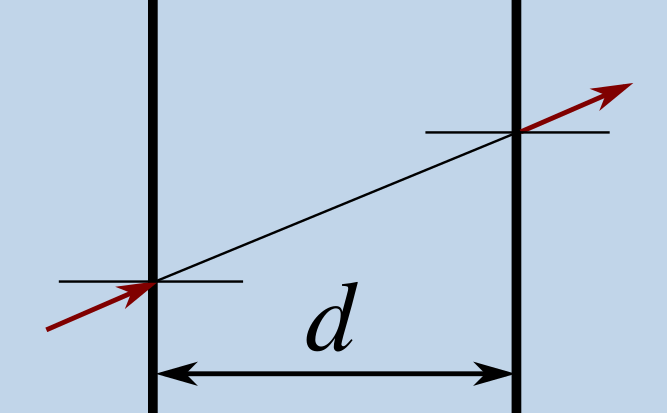
\includegraphics[width=0.8in]{slike/matrika_d.png}} & 
      $\begin{bmatrix} 1 & d\\  0 & 1 \end{bmatrix}$ \\ \hline

      Prehod preko meje dveh snovi & \parbox[c]{6em}{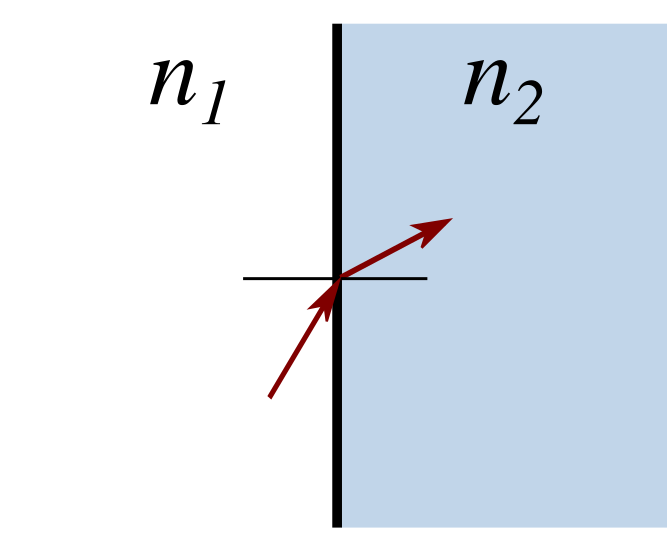
\includegraphics[width=0.8in]{slike/matrika_n.png}} & 
      $\begin{bmatrix} 1 & 0\\ 0 & \frac{n_{1}}{n_{2}} \end{bmatrix}$ \\ \hline
      
      Prehod preko konveksno ukrivljene meje $R>0$ & \parbox[c]{6em}{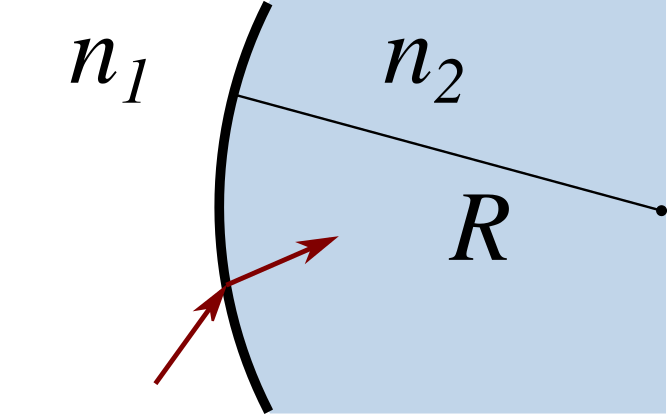
\includegraphics[width=0.8in]{slike/matrika_nR.png}} & 
      $\begin{bmatrix} 1 & 0\\ \frac{(n_{1}-n_{2})}{n_{2}R} & \frac{n_{1}}{n_{2}} \end{bmatrix}$ \\ \hline
      
      Prehod preko konveksne leče $f>0$ & \parbox[c]{6em}{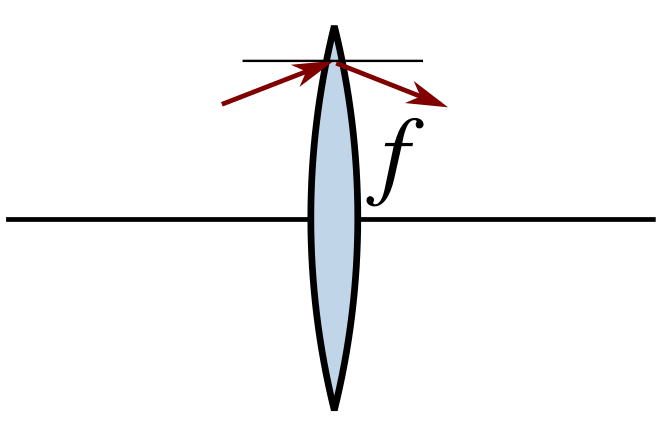
\includegraphics[width=0.8in]{slike/matrika_f.png}} & 
      $\begin{bmatrix} 1 & 0\\ -\frac{1}{f} & 1 \end{bmatrix}$ \\ \hline
      
      Odboj na konkavnem zrcalu $R>0$ & \parbox[c]{6em}{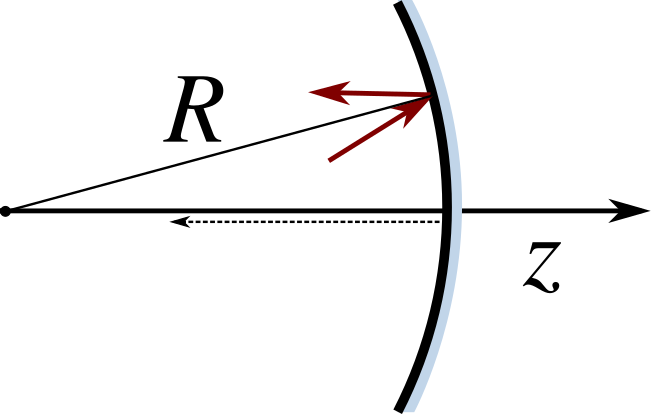
\includegraphics[width=0.8in]{slike/matrika_R.png}} & 
      $\begin{bmatrix} 1 & 0\\ -\frac{2}{R} & 1 \end{bmatrix}$ \\ \hline    
  \end{tabular}
  \caption{Matrike ABCD za nekaj osnovnih preslikav, ki veljajo tako v 
	  geometrijski optiki kot tudi za izračun preslikave kompleksnega
	  krivinskega radija $q$ Gaussovih snopov.}
\label{fig:Matrike-za-preslikave}
\end{table}

\begin{definition}
Pokaži, da za naslednje prehode veljajo ustrezne ABCD matrike. \\
\end{definition}
\begin{tabular}{|c|c|c|} \hline
  Opis prehoda & Skica & Matrika za prehod \\ \hline   
      Prehod skozi prostor in lečo & \parbox[c]{6em}{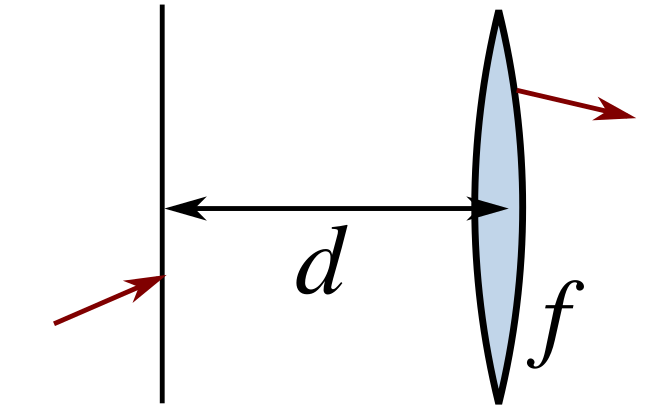
\includegraphics[width=0.8in]{slike/matrika_df.png}} & 
      $\begin{bmatrix} 1 & d\\ -\frac{1}{f} & 1-\frac{d}{f} \end{bmatrix}$ \\ \hline
      \parbox[c]{12em}{Prehod preko leče z debelino $d$ 
      in krivinskima radijema $R_1$ in $R_2$}& 
      \parbox[c]{6em}{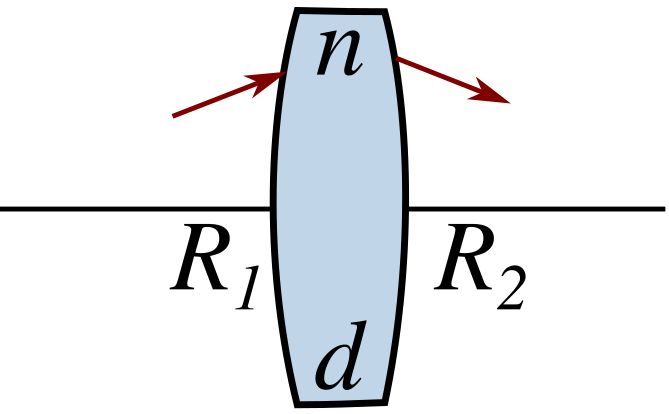
\includegraphics[width=0.8in]{slike/matrika_fd.png}} & 
      $\begin{bmatrix} 1-\frac{d}{nf_{1}} & \frac{d}{n}\\
      -\frac{1}{f_2}- \frac{1}{f_1}-\frac{d}{nf_1f_2}& 1-\frac{d}{nf_{2}} \end{bmatrix}$
      $f_{i}=\frac{R_{i}}{n-1}$\\ \hline
      Prehod čez zaporedje plasti & \parbox[c]{6em}{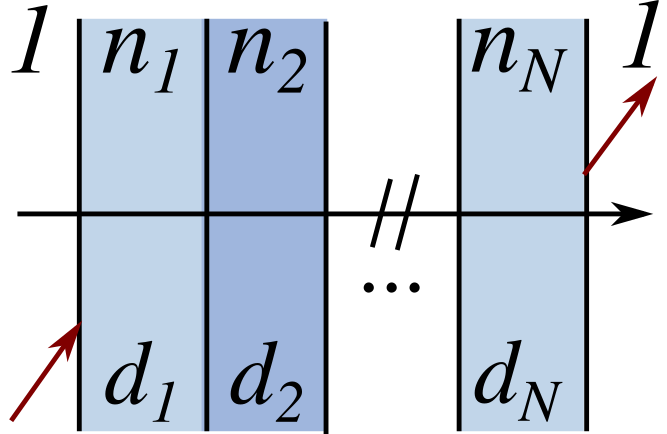
\includegraphics[width=0.8in]{slike/matrika_nN.png}} & 
      $\begin{bmatrix} 1 & \sum_{i=1}^{N}\frac{d_{i}}{n_{i}}\\ 0 & 1 \end{bmatrix}$ \\ \hline
   
  \end{tabular}
